\documentclass[25pt,margin=1in,innermargin=-4.5in,blockverticalspace=-0.25in]{tikzposter}
\geometry{paperwidth=39.37in,paperheight=39.37in}
\usepackage[utf8]{inputenc}
\usepackage{csquotes}
% \usepackage[estonian]{babel}
\usepackage{amsmath}
\usepackage{amsfonts}
\usepackage{amsthm}
\usepackage{amssymb}
\usepackage{mathrsfs}
\usepackage{graphicx}
\usepackage{adjustbox}
\usepackage{enumitem}
\usepackage{xcolor}
\usepackage[backend=biber,style=numeric]{biblatex}
\usepackage{unitartu-theme}
\usepackage{anyfontsize}
\usepackage{mwe} % for placeholder images

\renewenvironment{tikzfigure}[1][]{
\def \rememberparameter{#1}
\vspace{10pt}
\refstepcounter{figurecounter}
\begin{center}
}{
\ifx\rememberparameter\@empty
\else %nothing
\\[10pt]
%{\small Fig.~\thefigurecounter: \rememberparameter}
{\small \rememberparameter}
\fi
\end{center}
}


\addbibresource{refs.bib}

% set theme parameters
\tikzposterlatexaffectionproofoff
\usetheme{UniTartuTheme}
\usecolorstyle{UniTartuStyle}

\usepackage[scaled]{helvet}
\renewcommand\familydefault{\sfdefault} 
\renewcommand{\vec}[1]{\bm{#1}}
\newcommand{\Tr}{\text{Tr}}
\usepackage[T1]{fontenc}

\title{Microbial Community Richness along Temperature Gradients}
\author{\textbf{Danica Duan, Tom Clegg, Tom Smith, Samraat Pawar}
}
\institute{Life Science, Imperial College London \\}
\titlegraphic{
\includegraphics[width=0.18\linewidth]{figures/ic.png}}

% begin document
\begin{document}
\maketitle
\centering

\hspace{2.9em}
\begin{columns}
    \column{0.35}
    \block{Introduction}{
    \begin{itemize}
        \item Inconsistency of richness pattern with temperature reported in literature $^\cite{thompson2017communal}$. 
        \item The Earth Microbiome Project (EMP) reported a unimodel shape of community richness along temperature gradient $^\cite{hendershot2017consistently}$.
    \end{itemize}
    \begin{tikzfigure}[]
        \begin{tabular}{c@{}c@{}}
            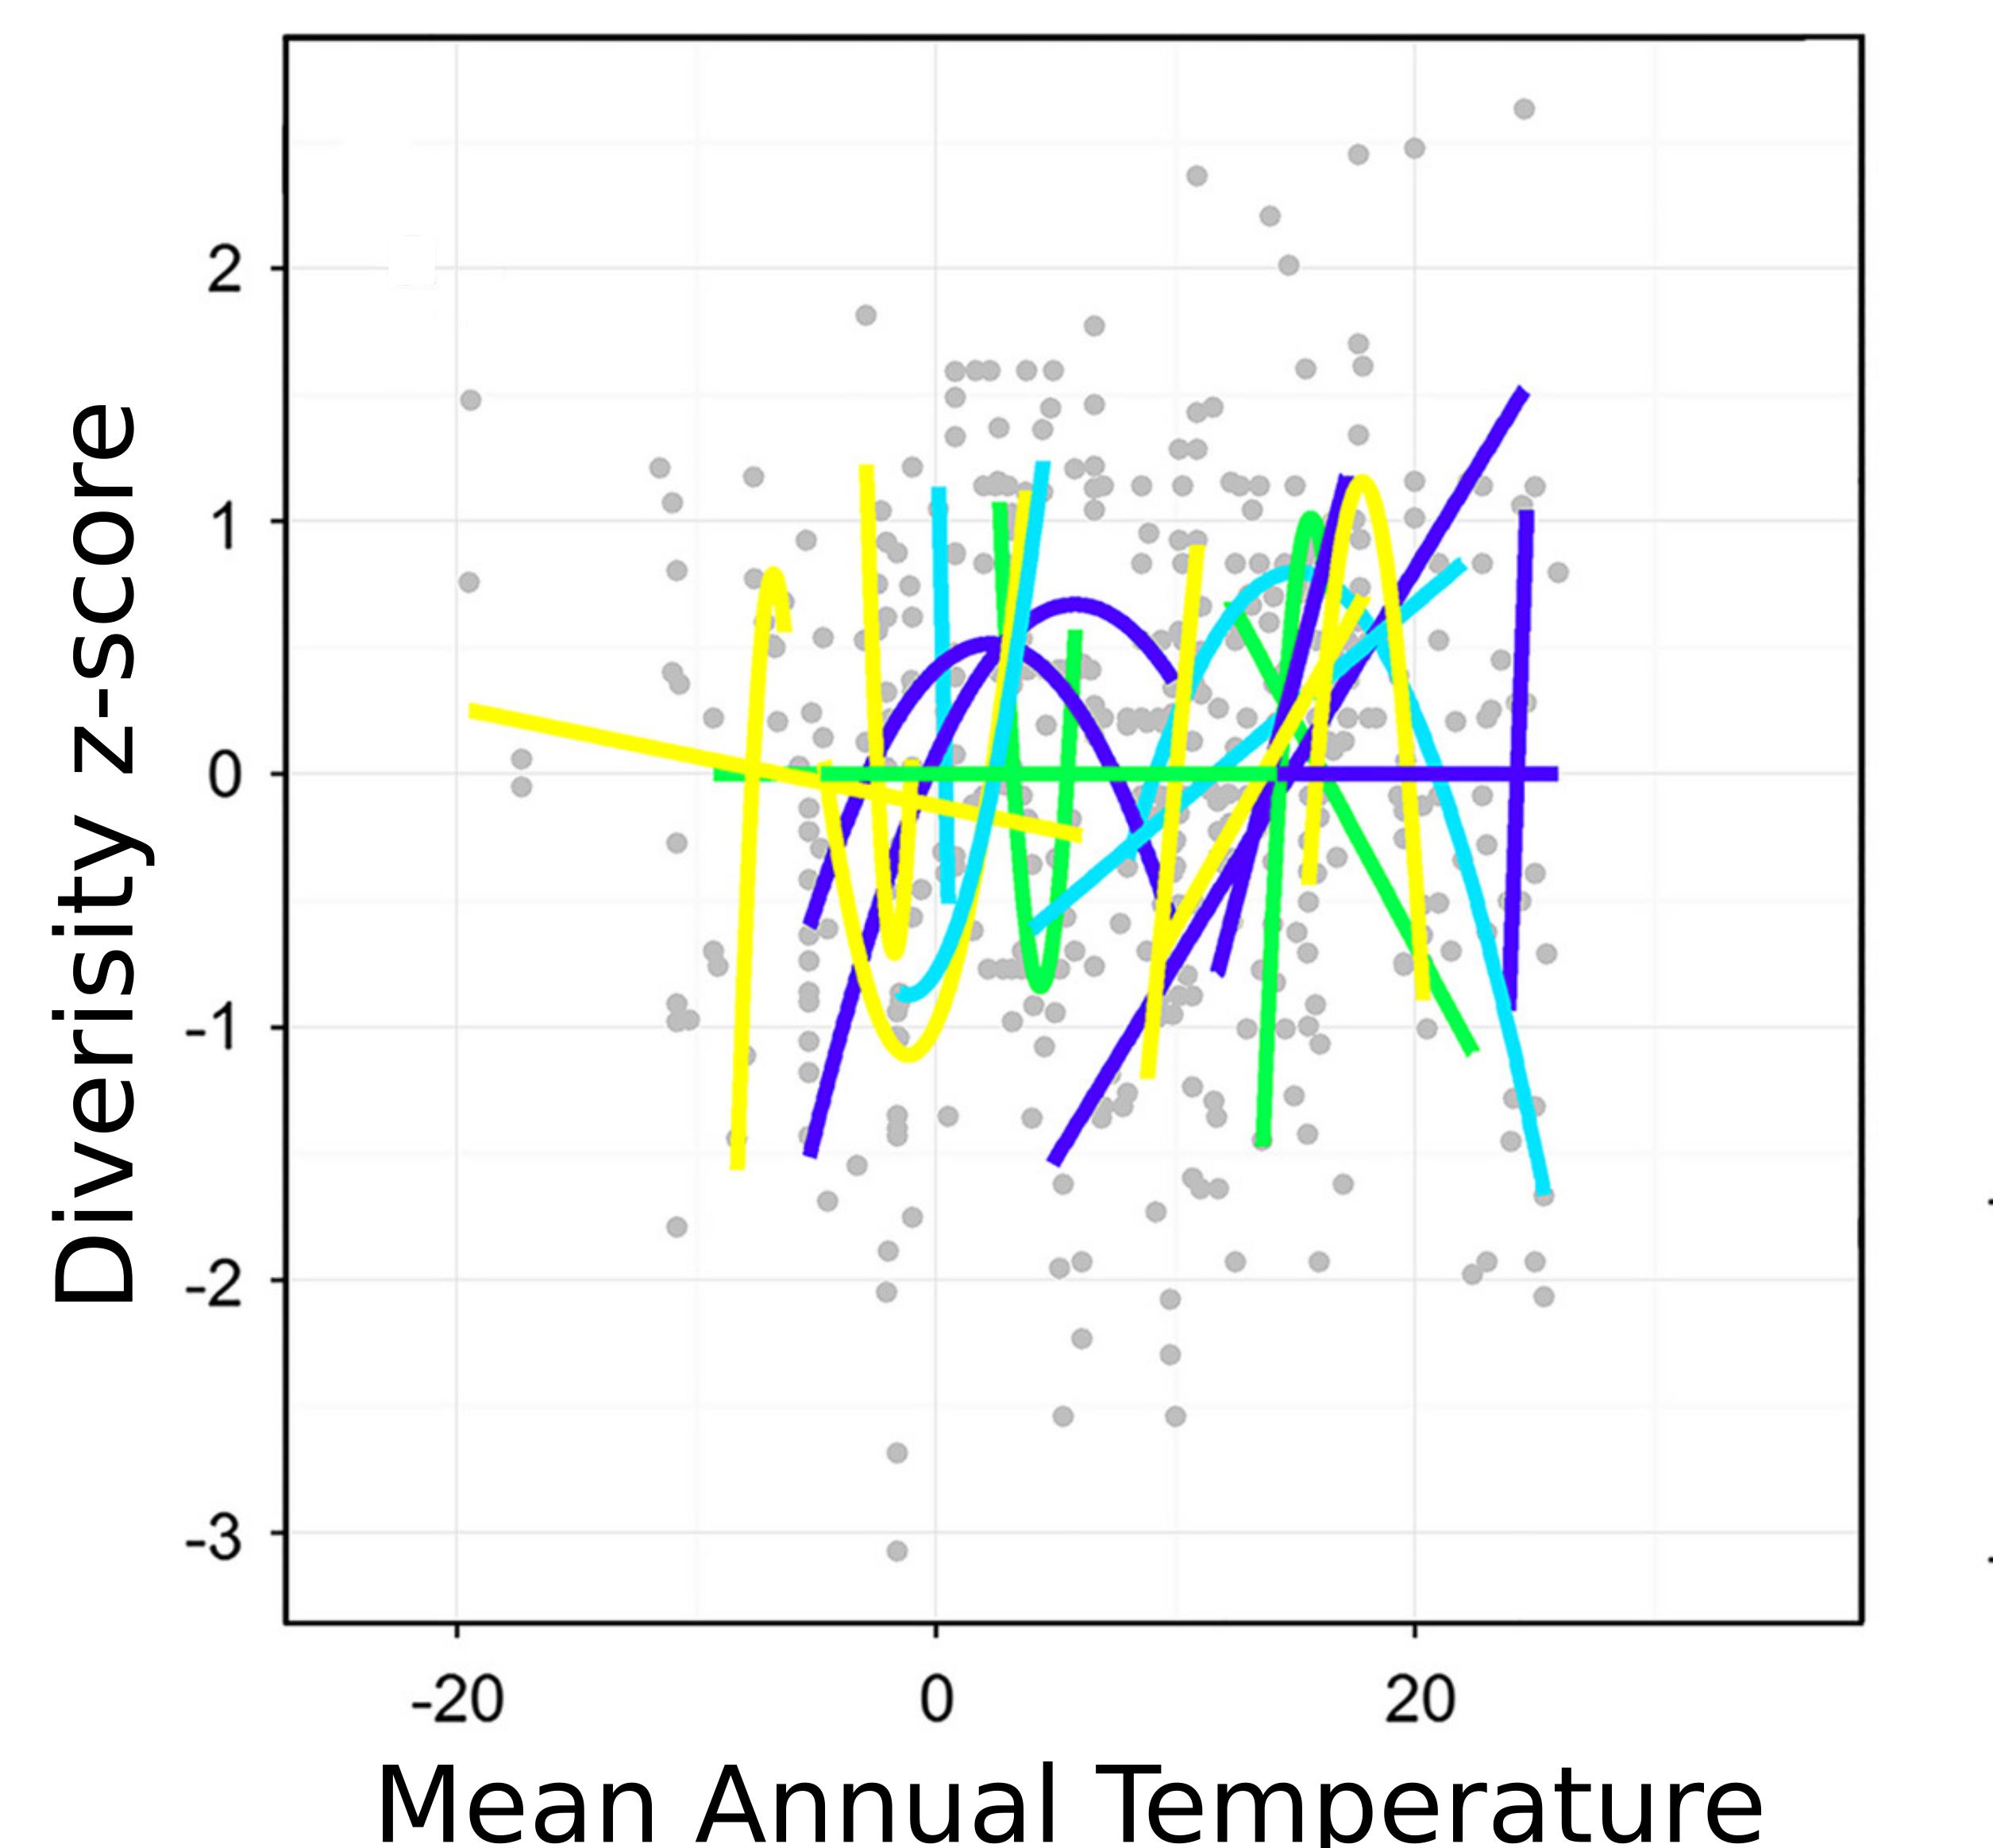
\includegraphics[scale=0.65]{figures/inconsistency.png}
            \hspace{0.5em}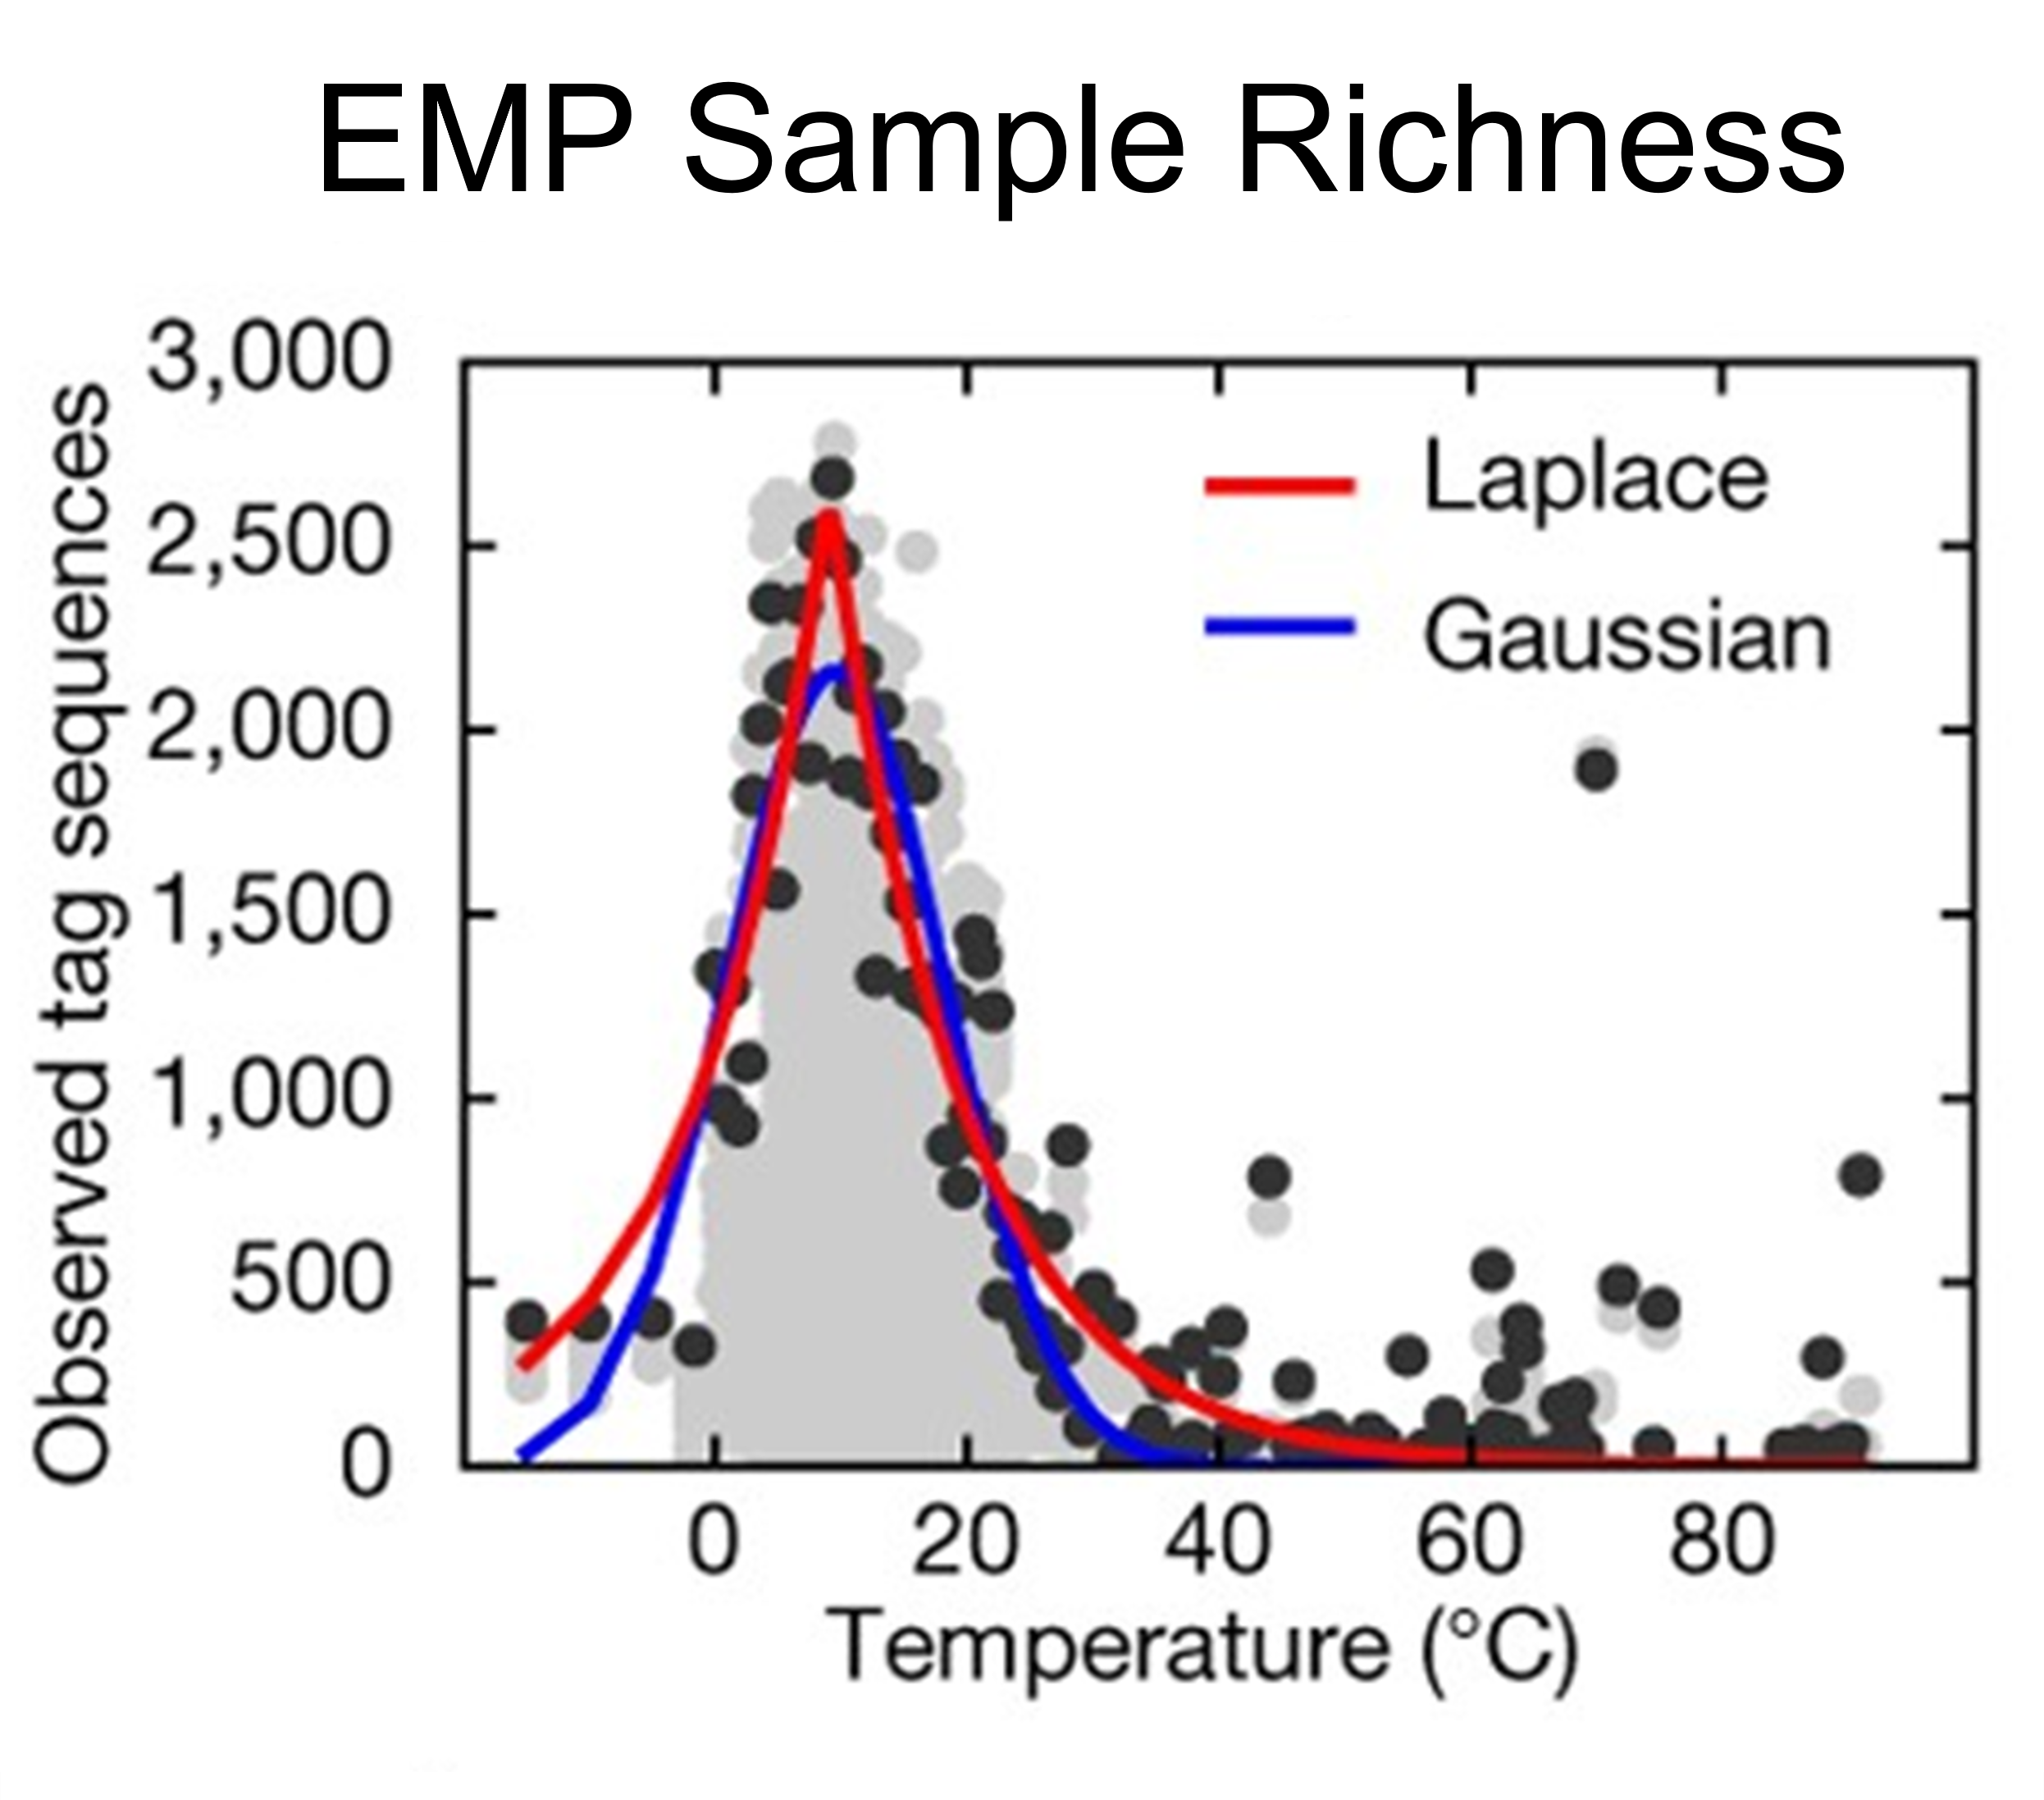
\includegraphics[scale=0.7]{figures/EMP.png}
        \end{tabular}
    \end{tikzfigure}
    }
    
    \block{Research Questions}{
    \vspace{1em}
    {\fontsize{32}{32}\selectfont 
    \textcolor{blue}{$P_1$.} The pattern of bacterial community richness along temperature gradients.
    
    \textcolor{blue}{$P_2$.} What determines the bacterial diversity patterns?}
    
    \vspace{1em}
    }

    \block{The Microbial Community Model $^\cite{marsland2020minimal}$}{
        \begin{align}
            \frac{dC_i}{dt} = C_i\Bigl(\sum_{\alpha=1}^{M}u_{i\alpha}(T)R_\alpha(1-\sum_{\beta=1}^{M}l_{\alpha \beta}) - m_i(T)\Bigl), \\
            \frac{dR_\alpha}{dt} = \rho_\alpha - \sum_{i=1}^{N}\Bigl(C_iu_{i\alpha}(T)R_\alpha-\sum_{\beta =1}^{M}C_iu_{i\beta}(T)R_\beta l_{\beta \alpha}\Bigl).
        \end{align}
        
        \begin{tikzfigure}[]
            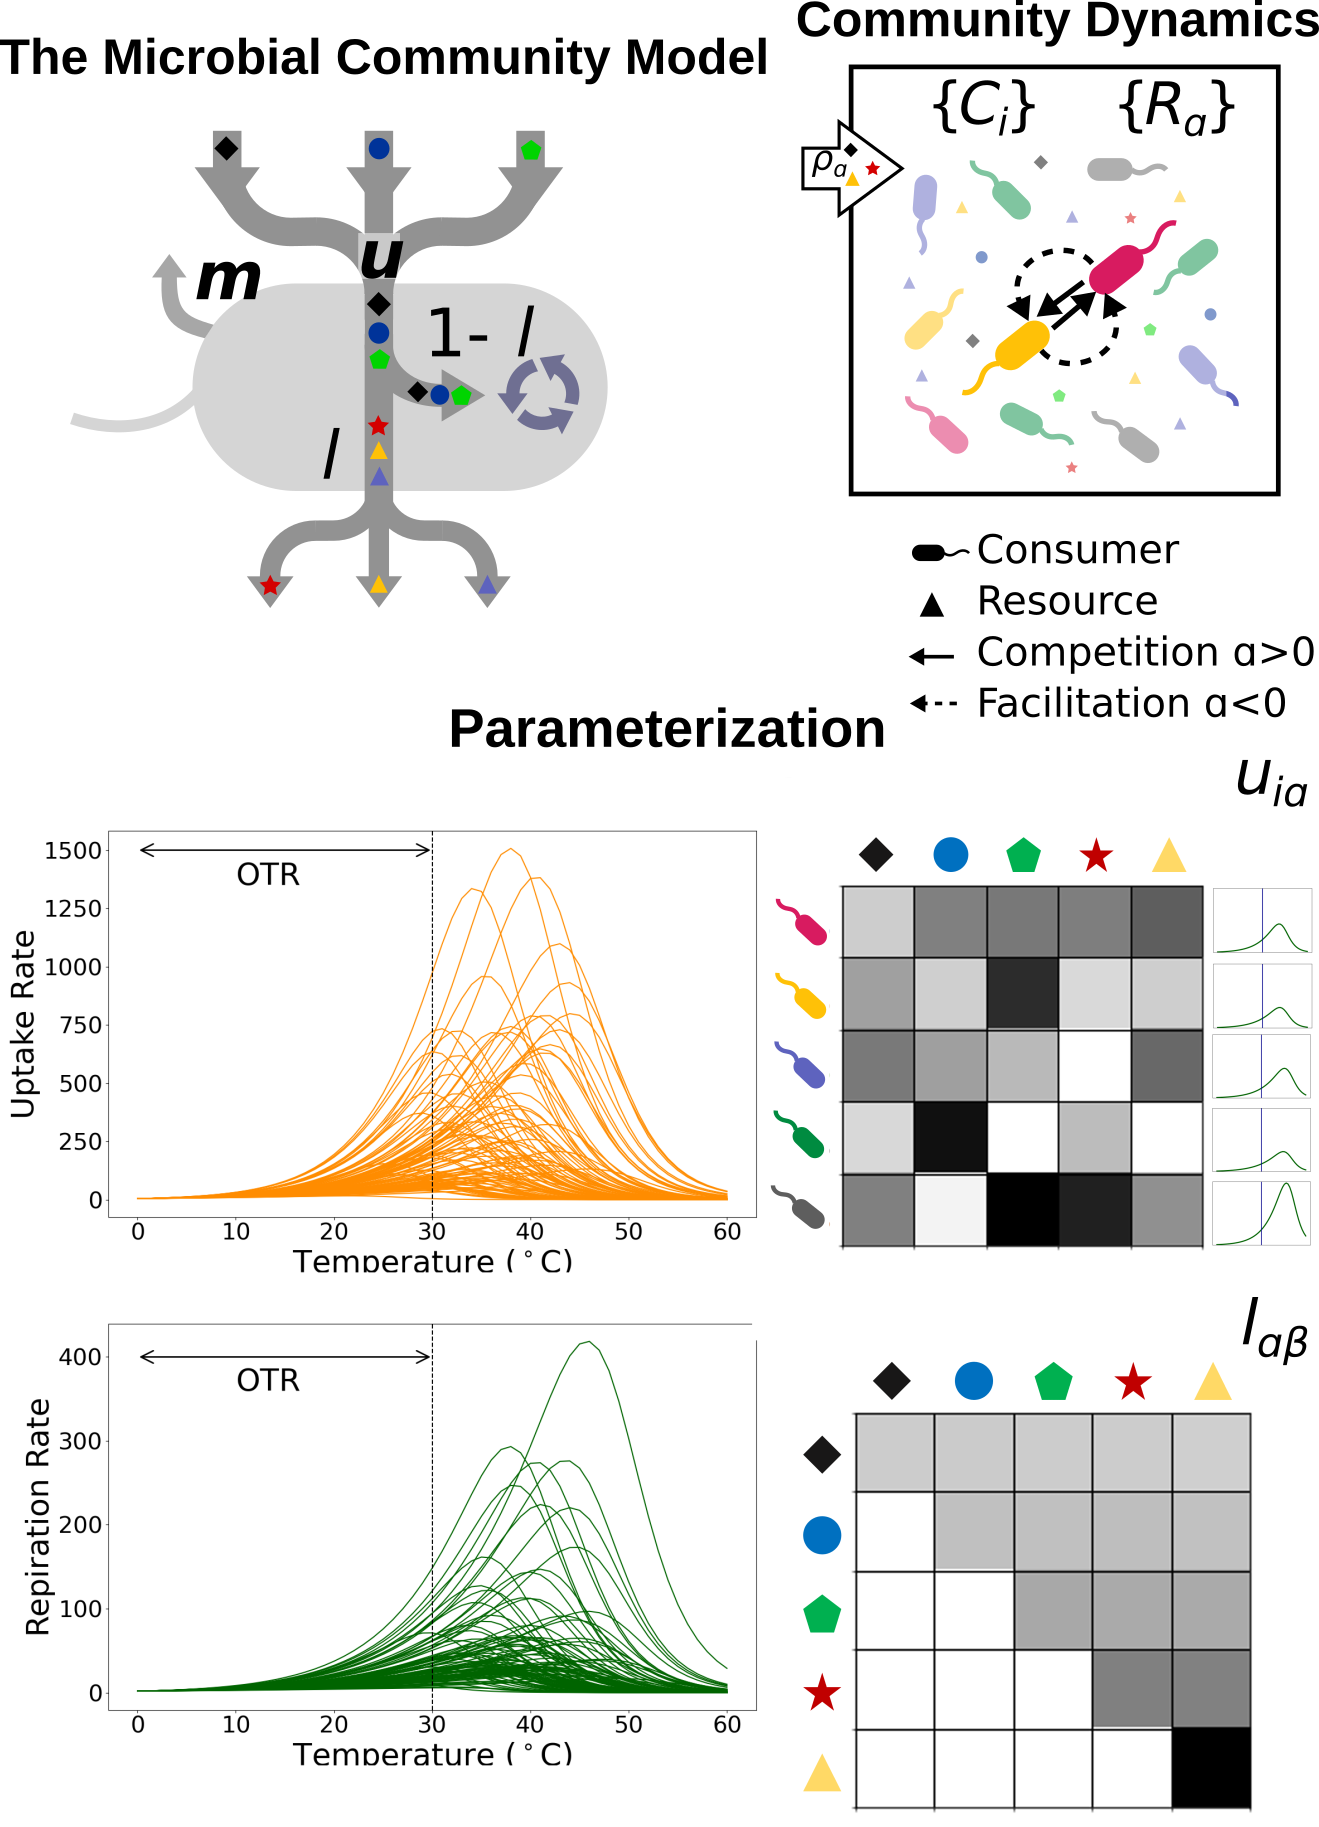
\includegraphics[width= 0.8\linewidth]{figures/MCM.png}
        \end{tikzfigure}
    }

    \column{0.35}
    \hspace{-3.4em}
    \block{Carbon Use Efficiency (CUE)}{
    \begin{itemize}
        \item Microbial CUE reflects species' metabolic strategies. 
        \item CUE is a function of temperature as the combination of metabolic rates.
    \end{itemize}
    \begin{equation*}
        CUE_i = \frac{\sum\limits _{j=1}^{M}U_{ij}S_j(1-\sum\limits_{k=1}^{M}l_{jk}) - R_i}{\sum\limits _{j=1}^{M}U_{ij}S_j}
    \end{equation*}
    \vspace{-1em}
    \begin{tikzfigure}[]
        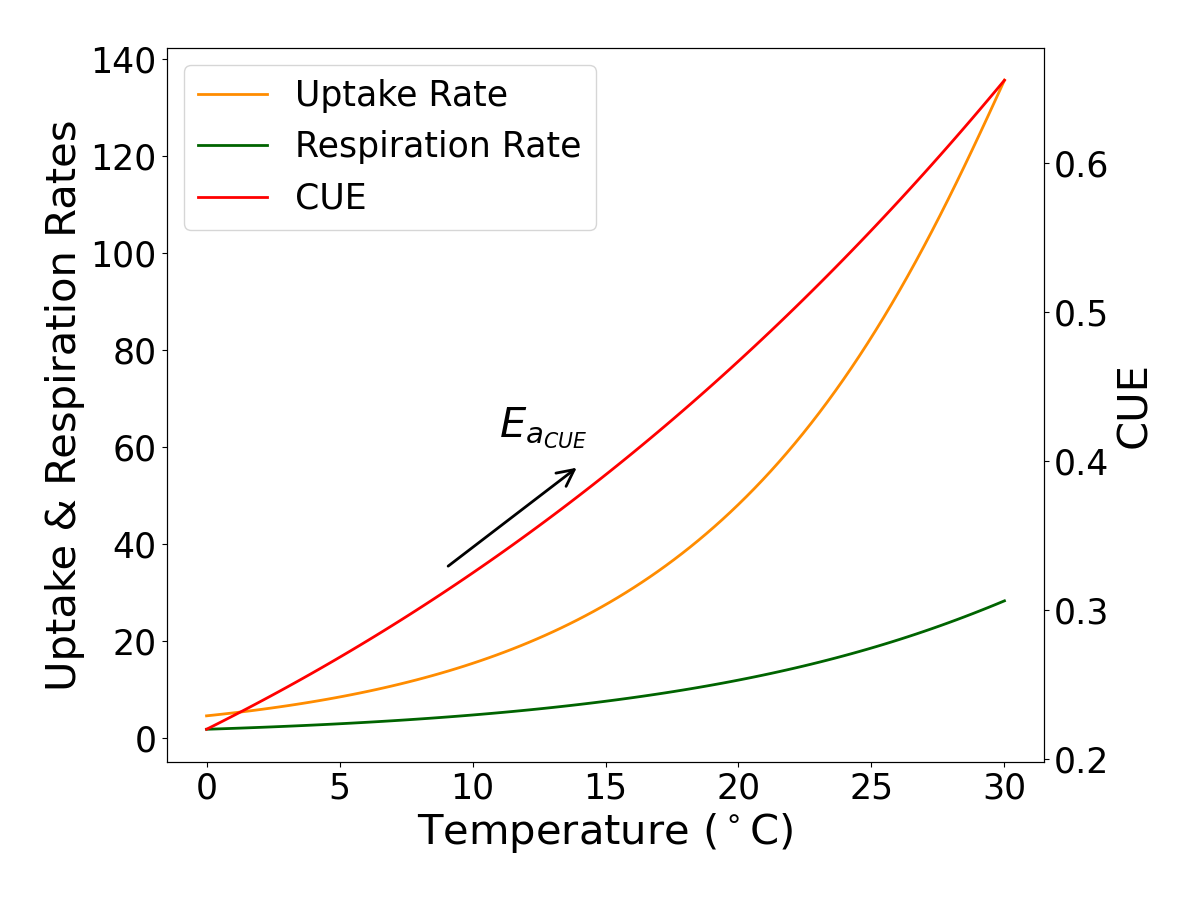
\includegraphics[width= 0.7\linewidth]{figures/URCUE.png}
    \end{tikzfigure}
    }
    
    \block{The Variation of Species CUE Reduces Community Richness}{
    By manipulating the covariance when randomly sampling normalization constants and activation energies for both uptake and respiration rates, we can reproduce all richness patterns: 
    \begin{tikzfigure}[]
        \begin{tabular}{c@{}c@{}c@{}}
        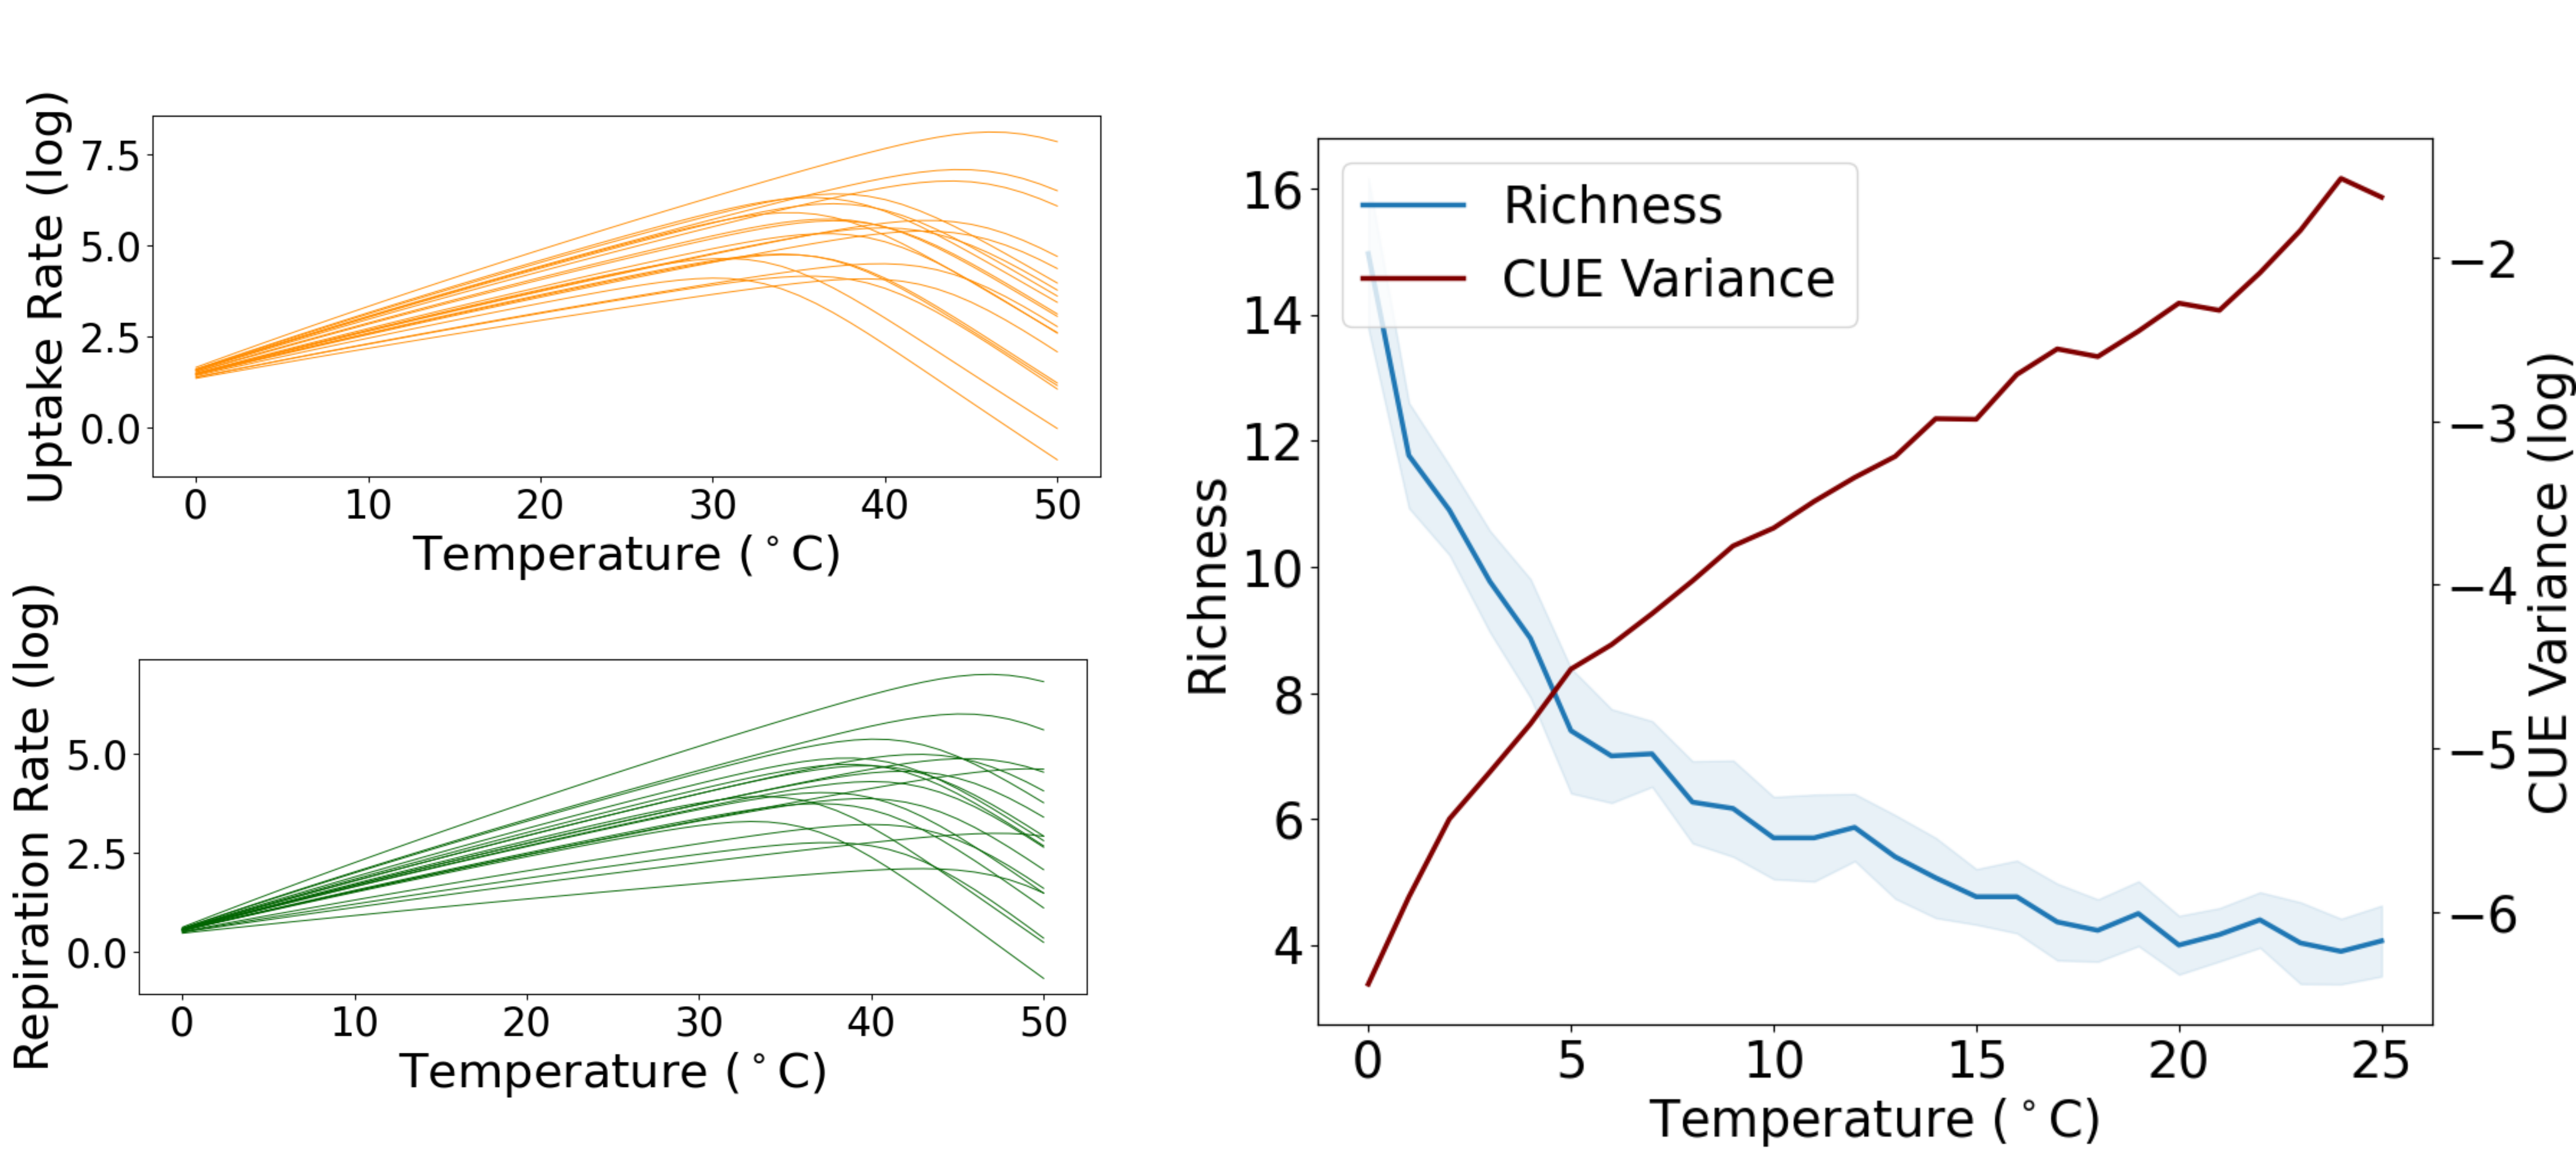
\includegraphics[width= 0.95\linewidth]{figures/1+1_rich.png} \\
        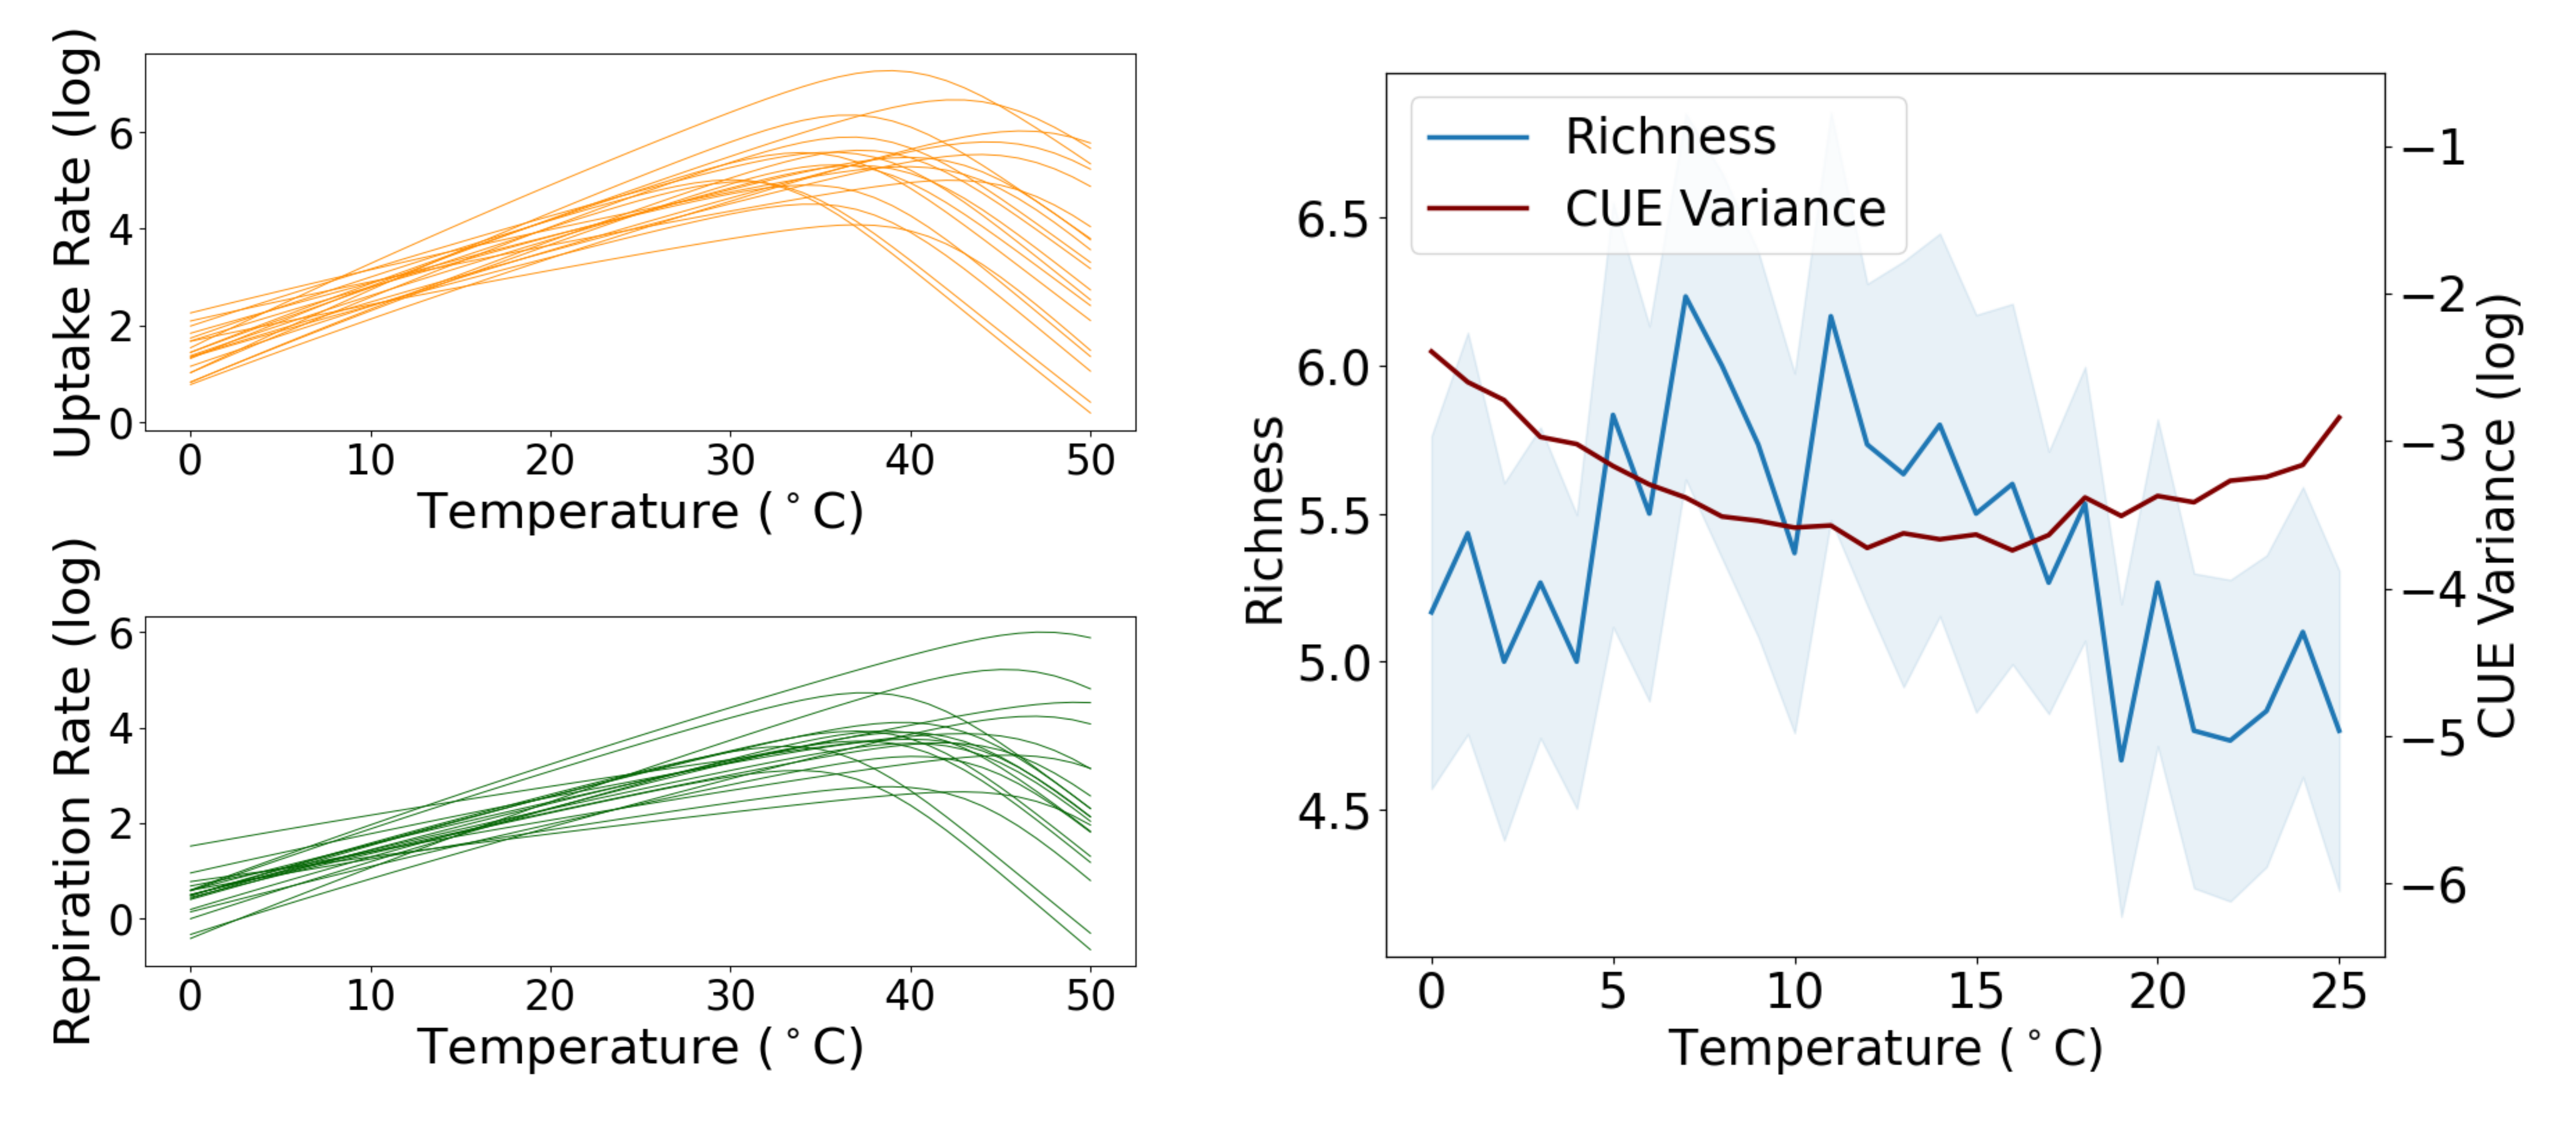
\includegraphics[width= 0.95\linewidth]{figures/0+0_rich.png} \\
        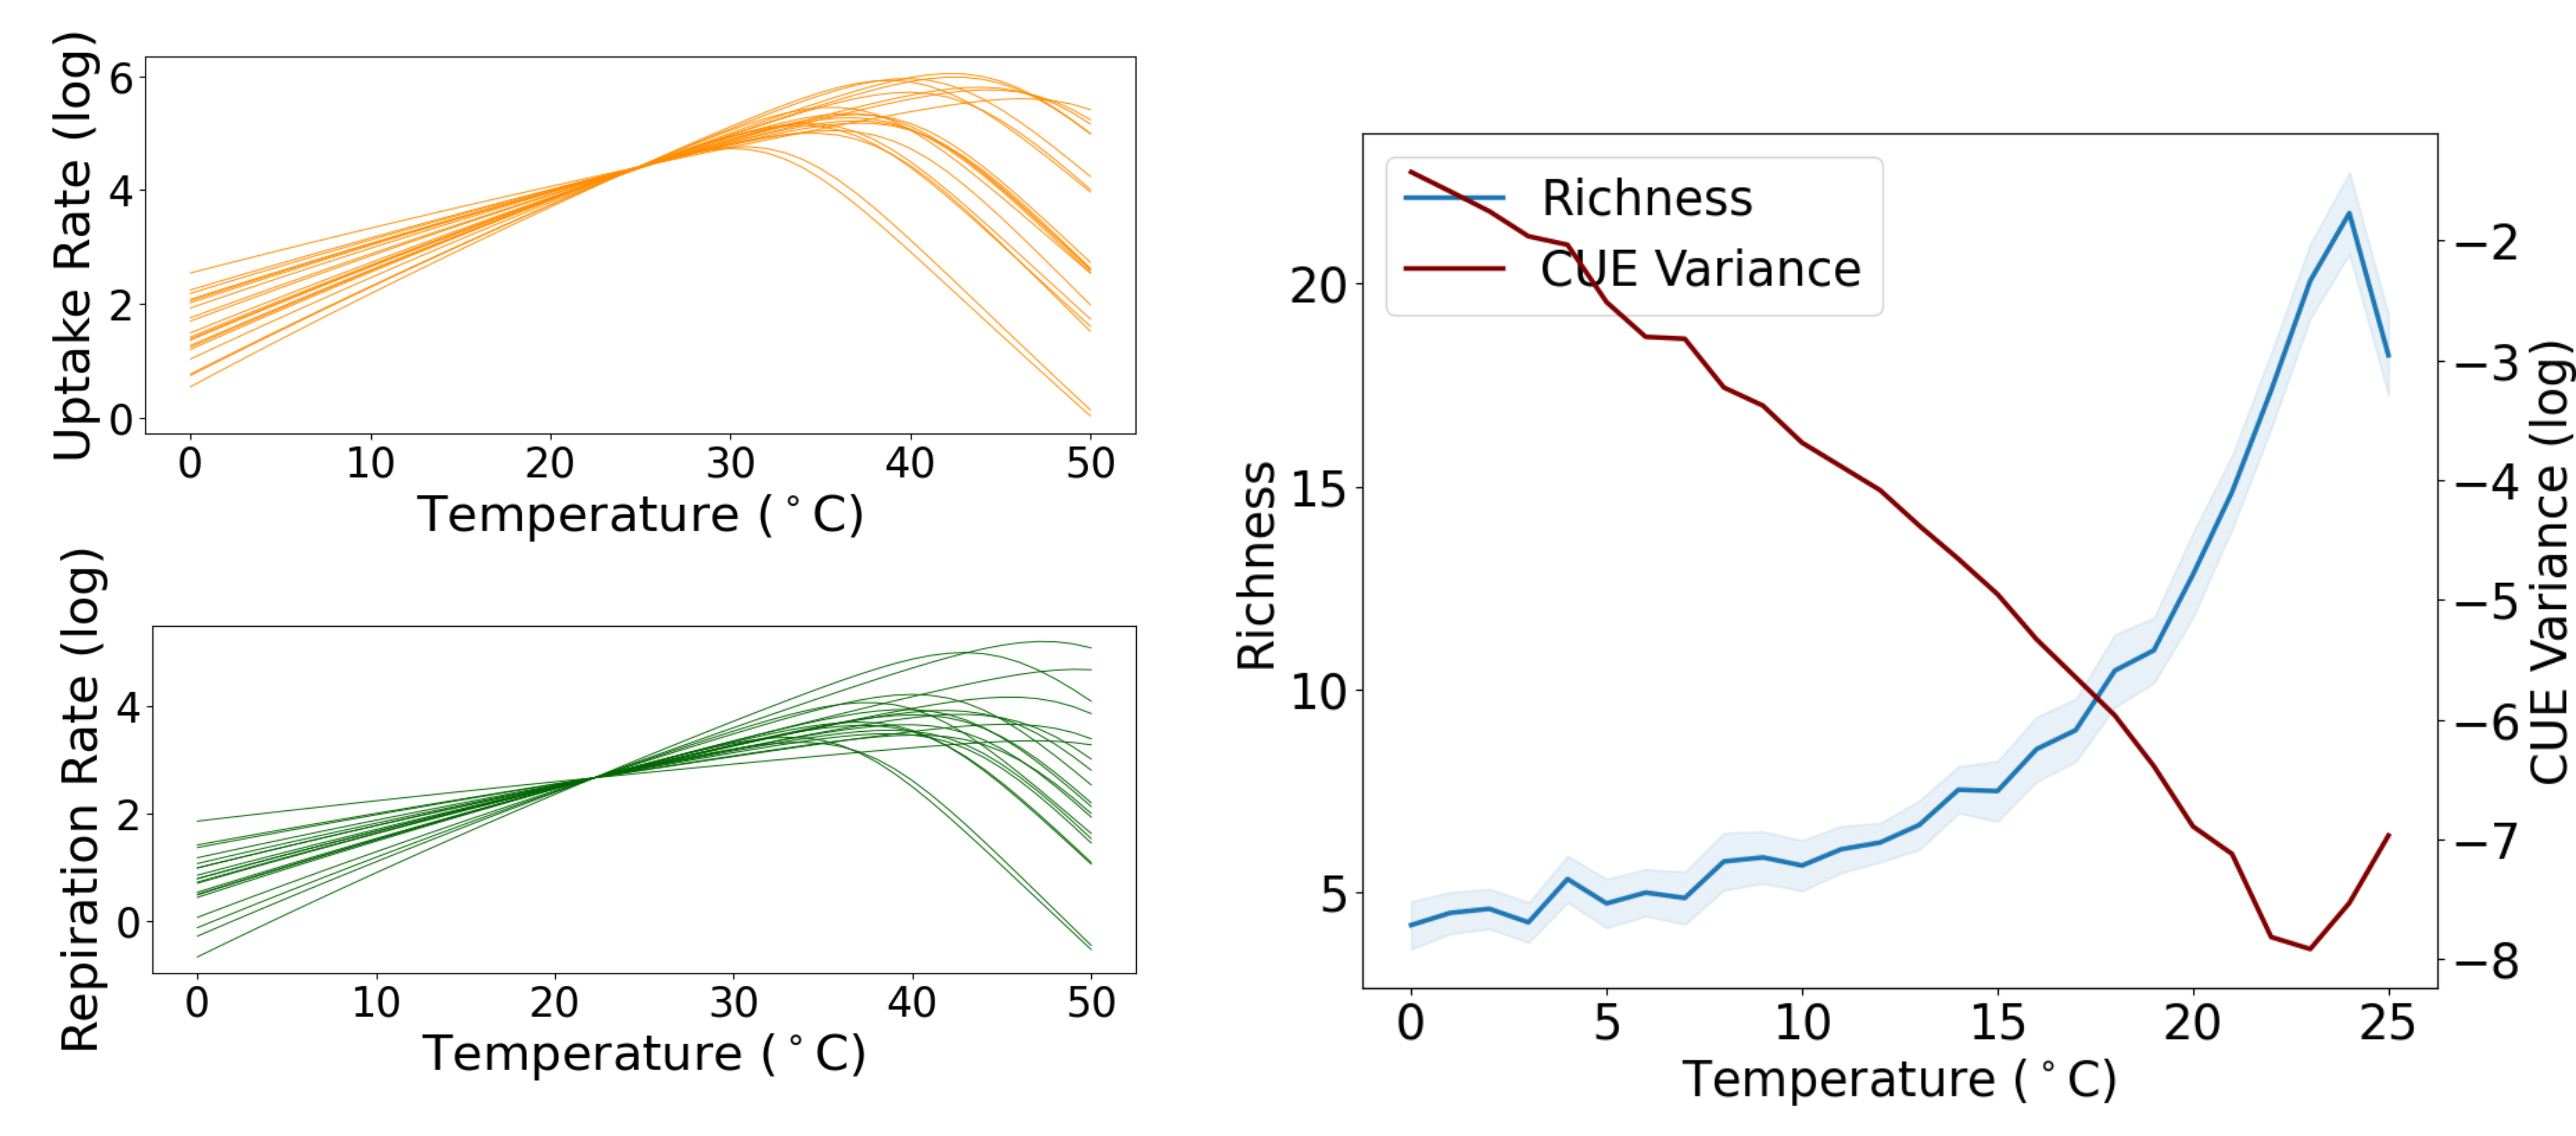
\includegraphics[width= 0.95\linewidth]{figures/-1+-1_rich.png}
        \end{tabular}
    \end{tikzfigure}
    }

    \column{0.3}
    \hspace{-3.7em}
    \block{Community Richness Increases along Temperature Gradients}{
        \begin{itemize}
        \item Community richness increases as the variation of CUE is reduced at higher temperature.
        \vspace{-0.85em}
            \begin{tikzfigure}[]
                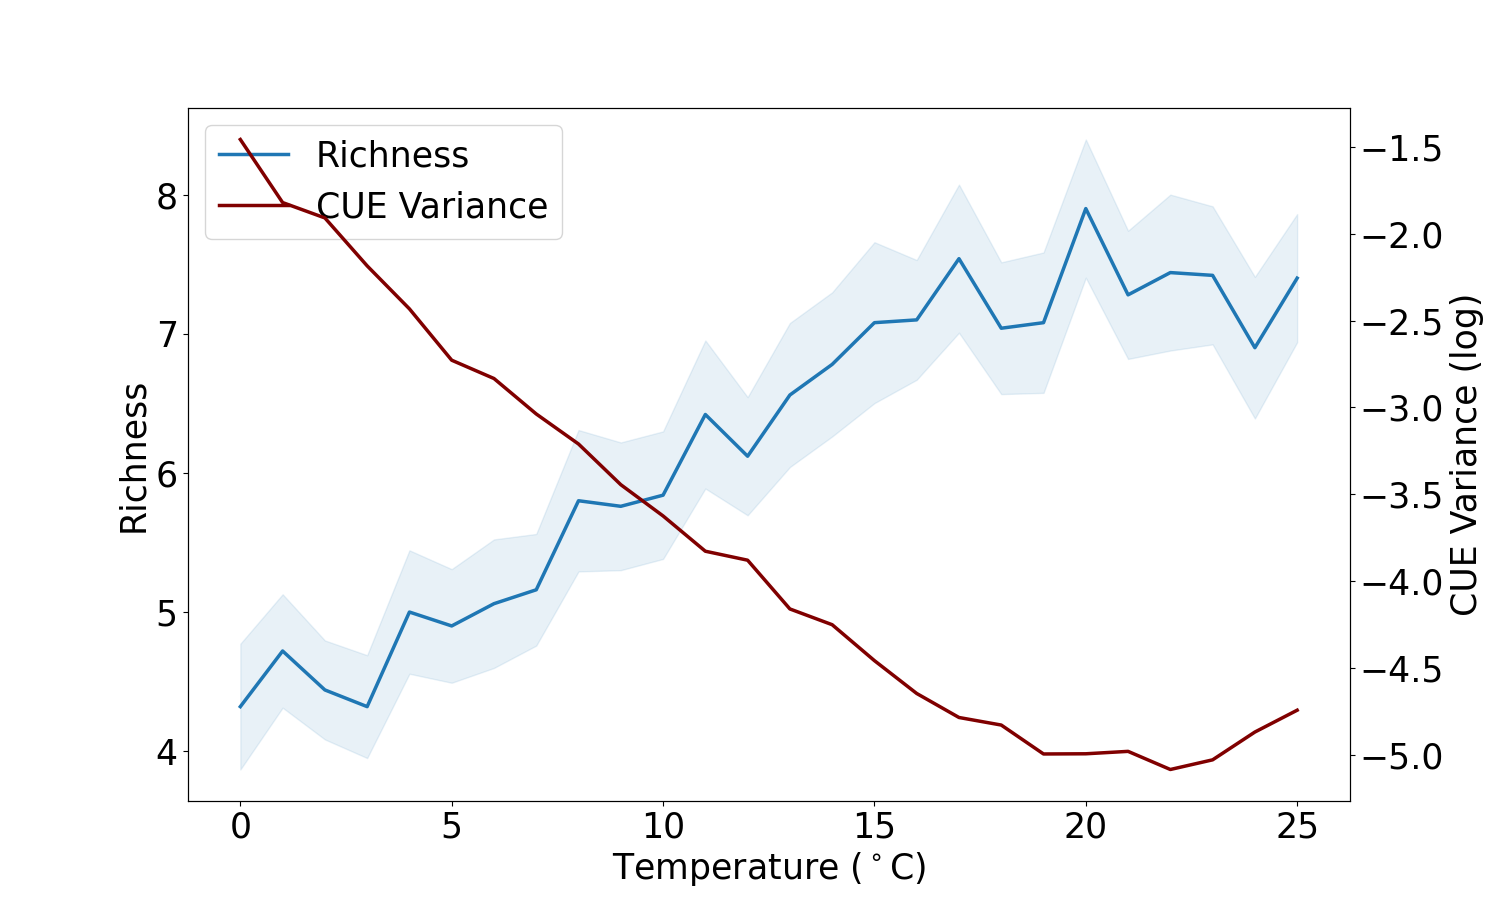
\includegraphics[width=\linewidth]{figures/rich_varCUE_temp.png}
            \end{tikzfigure}
        
        \item Species with lower uptake are higher respiration rates are favored in species sorting.
        \vspace{-0.85em}
            \begin{tikzfigure}[]
                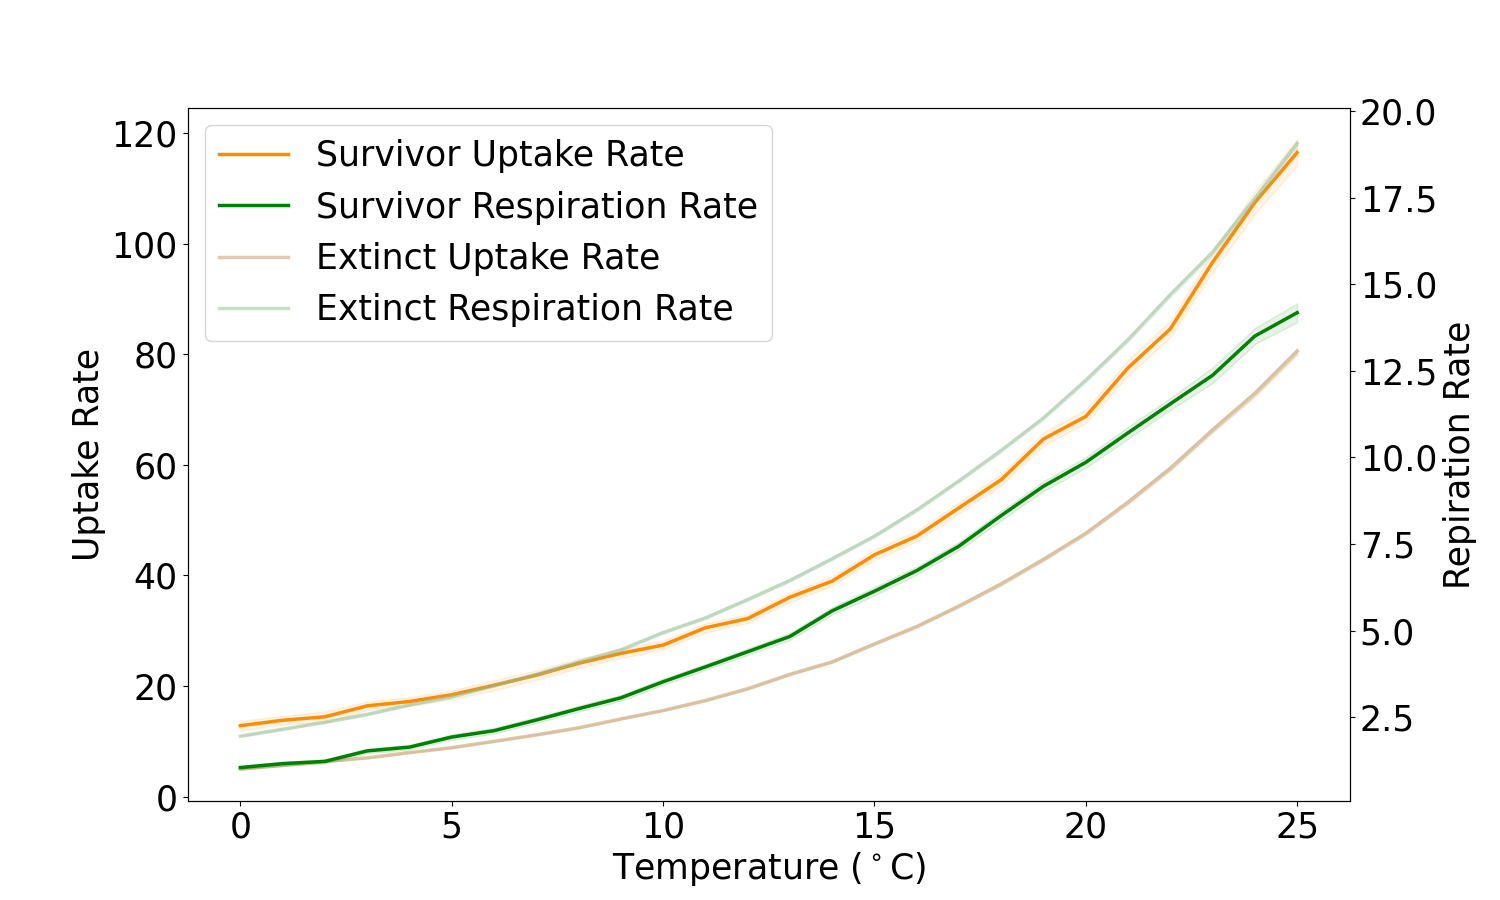
\includegraphics[width=\linewidth]{figures/U+R_temp.png}
            \end{tikzfigure}
        
        \item Species with higher CUE are favored at all temperatures.
        \vspace{-0.85em}
            \begin{tikzfigure}[]
                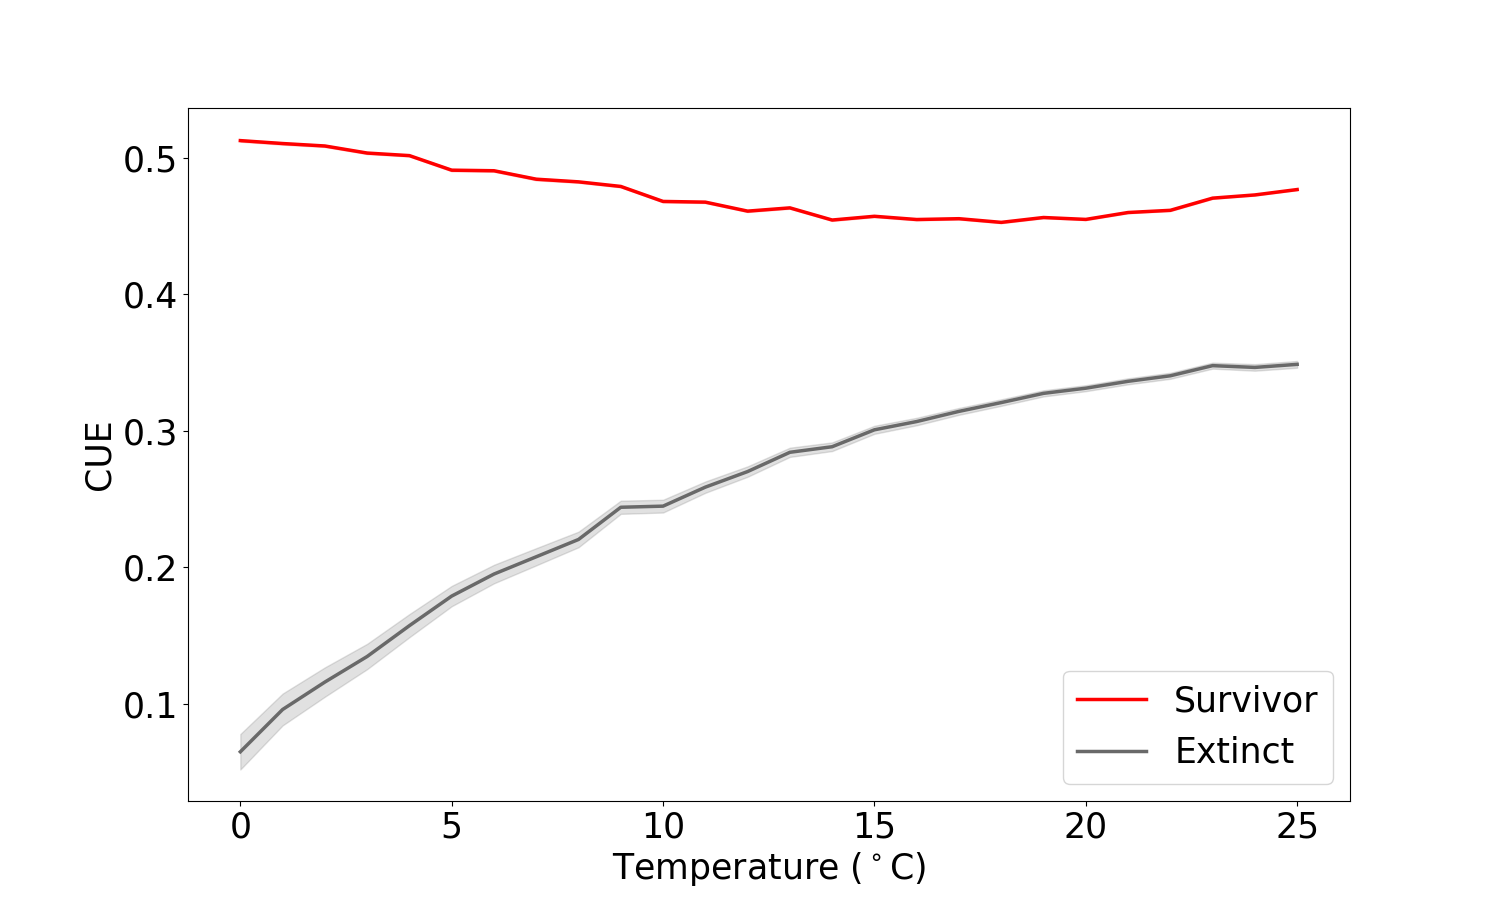
\includegraphics[width=\linewidth]{figures/CUE_temp.png}
            \end{tikzfigure}
            \end{itemize}

    }
    \block{Conclusions}{
        {\fontsize{32}{32}\selectfont 
    \begin{itemize}
        \item Species richness are higher in communities assembled at higher temperatures.  \textcolor{blue}{\leftarrow $P_1$}
        \item This increase is driven by the declining variation of species' metabolic strategies in the community. \textcolor{blue}{\leftarrow $P_2$}
        \item Higher resource utilization ability in all assembled communities as a result of species sorting. 
    \end{itemize}}
    }

    \block{{\fontsize{34}{34}\selectfont References}}{
    \vspace{-0.6em}
        \renewcommand*{\bibfont}{\normalfont\footnotesize}
        \printbibliography[heading=none]
    }
\end{columns}

\end{document}